\section{Introduction}


\begin{frame}{Introduction}\framesubtitle{Édition collaborative}

  L'édition collaborative concerne toutes les activités effectuées en
  \textbf{groupe} dans le but de produire un \textbf{document}. L'effort
  collectif permet de bénéficier de multiples points de vues différents.

  \begin{itemize}
  \item[$\rightarrow$] Les documents sont de \textbf{meilleure qualité}.
  \end{itemize}
  
  \vfill

  \noindent
  \begin{minipage}{0.6\textwidth}
    \textit{Le Wikipédia anglais compte \textbf{5 millions} d'articles,
      \textbf{40 millions} de pages et \textbf{112 milles} utilisateurs
      actifs.\\Les articles possèdent une \textbf{fiabilité} \textbf{comparable}
      à celle de l'Encyclopædia Britannica \REF.}

  \end{minipage}
  \hfill
  \begin{minipage}{0.3\textwidth}
    \begin{figure}
      \begin{center}
        
\includegraphics[width=0.7\textwidth]{img/wikipedia.png}
      \end{center}
    \end{figure}
  \end{minipage}
 

\end{frame}


\begin{frame}{slide google docs}
  todo
\end{frame}

\begin{frame}{Introduction}\framesubtitle{Éditeur collaboratif}
  \begin{figure}
    \begin{center}
      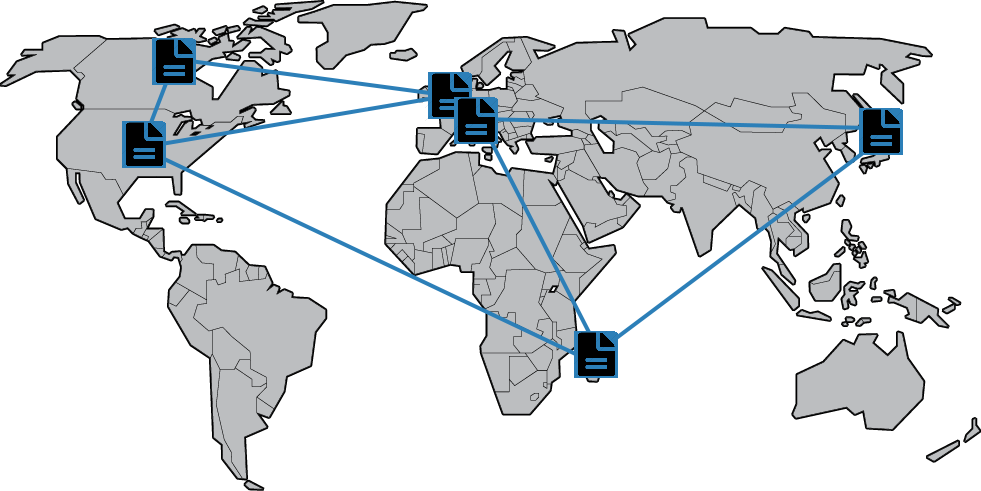
\includegraphics[width=0.8\textwidth]{img/world.png}
    \end{center}
  \end{figure}

  \begin{itemize}
  \item Répartition géographique des collaborateurs;
  \item Édition en temps réel.
  \end{itemize}
\end{frame}


%%% Local Variables:
%%% mode: latex
%%% TeX-master: "../slides"
%%% End:
